\documentclass[xetex,mathserif,serif]{beamer}
\usepackage{polyglossia}
\setdefaultlanguage[babelshorthands=true]{russian}
\usepackage{minted}
\usepackage{tabu}

\useoutertheme{infolines}

\usepackage{fontspec}
\setmainfont{FreeSans}
\newfontfamily{\russianfonttt}{FreeSans}

\setbeamertemplate{blocks}[rounded][shadow=false]
\setbeamercolor*{block title example}{fg=green!50!black,bg=green!20}
\setbeamercolor*{block body example}{fg=black,bg=green!10}

\setbeamercolor*{block title alerted}{fg=red!50!black,bg=red!20}
\setbeamercolor*{block body alerted}{fg=black,bg=red!10}

\tabulinesep=0.7mm

\title{Диаграммы классов UML}
\author[Юрий Литвинов]{Юрий Литвинов \newline \textcolor{gray}{\small\texttt{yurii.litvinov@gmail.com}}}

\date{22.03.2017г}

\begin{document}
	
	\frame{\titlepage}

	\section{Domain-Driven Design: анализ}

	\begin{frame}
		\frametitle{Domain-Driven Design}
		\textbf{Domain-Driven Design} --- модная нынче методология проектирования, использующая предметную область как основу архитектуры системы
		\begin{itemize}
			\item Архитектура приложения строится вокруг \textbf{Модели предметной области}
			\item Модель определяет \textbf{Единый язык}, на котором общаются и разработчики, и эксперты, описывая естественными фразами то, что происходит и в программе, и в реальности
			\item Модель --- это не только диаграммы, это ещё (и прежде всего) код, и устное общение
		\end{itemize}
		Причём тут UML --- DDD даёт ответ на вопрос ``откуда брать эти все классы'' и позволяет целенаправленно уточнять и улучшать модель. 
		Особенно полезно, когда предметная область не очень знакома (как будет в домашке).
	\end{frame}

	\begin{frame}
		\frametitle{Книжка}
		Эрик Эванс, ``Предметно-ориентированное проектирование. Структуризация сложных программных систем''. М., ``Вильямс'', 2010, 448 стр.
		\begin{center}
			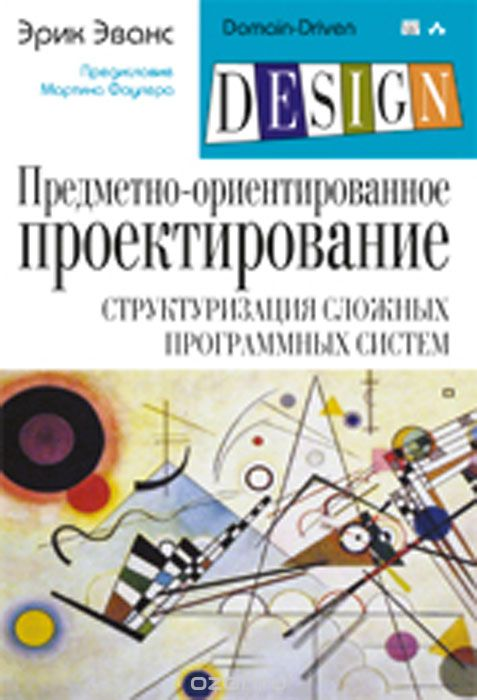
\includegraphics[width=0.25\textwidth]{dddCover.jpg}
		\end{center}
	\end{frame}

	\begin{frame}
		\frametitle{Domain-Driven Design, анализ}
		\framesubtitle{Пример: печатные платы}
		\begin{center}
			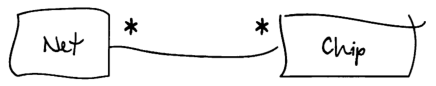
\includegraphics[width=0.6\textwidth]{netClasses.png}

			\bigskip

			\bigskip
			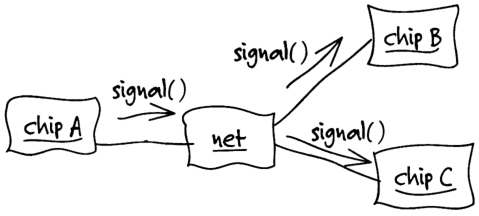
\includegraphics[width=0.6\textwidth]{netObjects.png}
		\end{center}
	\end{frame}

	\begin{frame}
		\frametitle{Печатные платы, топология}
		\begin{center}
			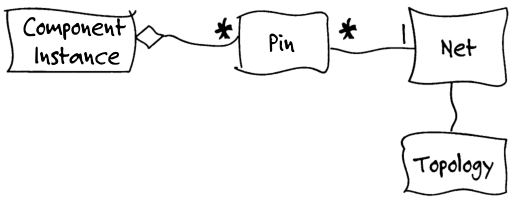
\includegraphics[width=0.7\textwidth]{topology.png}
		\end{center}
	\end{frame}

	\begin{frame}
		\frametitle{Печатные платы, сигналы}
		\begin{center}
			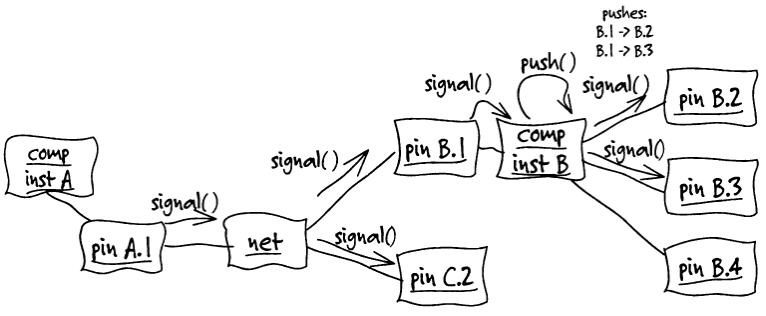
\includegraphics[width=0.9\textwidth]{signals.png}
		\end{center}
	\end{frame}

	\begin{frame}
		\frametitle{Печатные платы, прозванивание}
		\begin{center}
			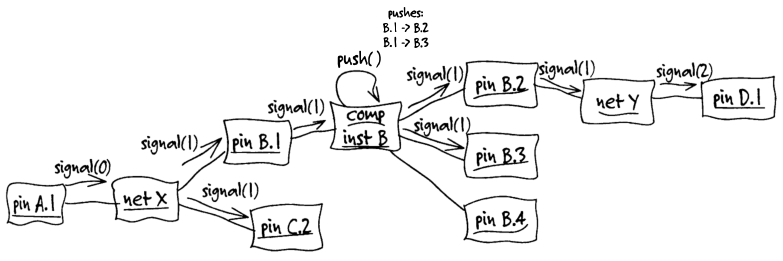
\includegraphics[width=\textwidth]{probeSimulation.png}
		\end{center}
	\end{frame}

	\begin{frame}
		\frametitle{Печатные платы, типы}
		\begin{center}
			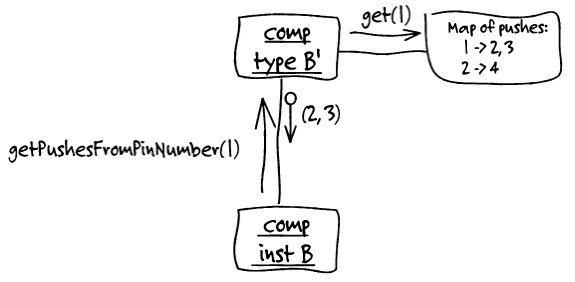
\includegraphics[width=0.7\textwidth]{types.png}
		\end{center}
	\end{frame}

	\begin{frame}
		\frametitle{Печатные платы, модель}
		\begin{center}
			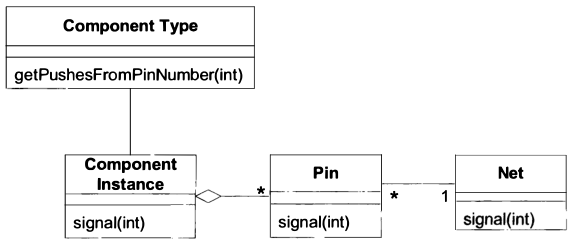
\includegraphics[width=0.8\textwidth]{finalModel.png}
		\end{center}
	\end{frame}

	\begin{frame}
		\frametitle{Выводы: правила игры}
		\begin{itemize}
			\item Детали реализации не участвуют в модели
			\begin{itemize}
				\item ``База данных? Какая база данных?''
			\end{itemize}
			\item Должно быть можно общаться, пользуясь только именами классов и методов
			\item Не нужные для текущей задачи сущности предметной области не должны быть в модели
			\item Могут быть скрытые сущности, которые следует выделить явно
			\begin{itemize}
				\item при этом объяснив экспертам их роль в реальной жизни и послушав их мнение
				\item например, различные ограничения могут стать отдельными классами
			\end{itemize}
			\item Диаграммы объектов могут быть очень полезны
		\end{itemize}
	\end{frame}

	\section{CASE-системы}

	\begin{frame}
		\frametitle{Computer-Aided Software Engineering}
		\begin{itemize}
			\item В 80-е годы термином CASE называли всё, что помогает разрабатывать ПО с помощью компьютера
			\begin{itemize}
				\item Даже текстовые редакторы
			\end{itemize}
			\item Теперь --- прежде всего средства для визуального моделирования (UML-диаграммы, ER-диаграммы и т.д.)
			\item Отличаются от графических редакторов тем, что ``понимают'', что в них рисуют
			\item Нынче чаще используются термины ``MDE tool'', ``UML tool'' и т.д.
		\end{itemize}
	\end{frame}

	\begin{frame}
		\frametitle{Типичная функциональность CASE-инструментов}
		\begin{itemize}
			\item Набор визуальных редакторов
			\item Репозиторий
			\item Набор генераторов
			\item Текстовый редактор
			\item Редактор форм
			\item Средства обратного проектирования (reverse engineering)
			\item Средства верификации и анализа моделей
			\item Средства эмуляции и отладки
			\item Средства обеспечения командной разработки
			\item API для интеграции с другими инструментами
			\item Библиотеки шаблонов и примеров
		\end{itemize}
	\end{frame}

	\begin{frame}
		\frametitle{Примеры CASE-инструментов}
		\begin{itemize}
			\item ``Рисовалки''
			\begin{itemize}
				\item Visio
				\item Dia
				\item SmartDraw
				\item Creately
			\end{itemize}
			\item Полноценные CASE-системы
			\begin{itemize}
				\item Enterprise Architect
				\item Rational Software Architect
				\item MagicDraw
				\item Visual Paradigm
				\item GenMyModel
			\end{itemize}
			\item Забавные штуки
			\begin{itemize}
				\item \url{https://www.websequencediagrams.com/}
				\item \url{http://yuml.me/}
				\item \url{http://plantuml.com/}
			\end{itemize}
		\end{itemize}
	\end{frame}

	\section{Диаграммы классов и объектов UML}

	\begin{frame}
		\frametitle{Диаграммы классов UML}
		\begin{center}
			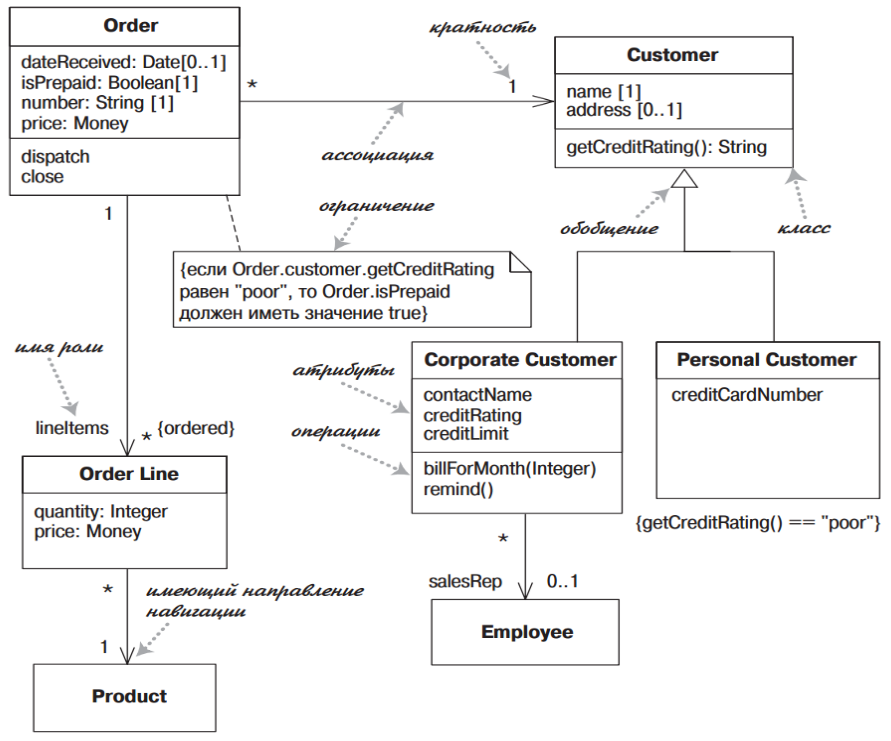
\includegraphics[width=0.7\textwidth]{umlClassDiagram.png}
		\end{center}
	\end{frame}

	\begin{frame}
		\frametitle{Свойства}
		\begin{columns}
			\begin{column}{0.3\textwidth}
				\begin{center}
					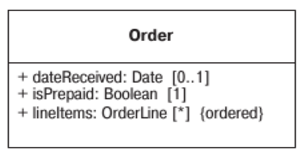
\includegraphics[width=0.8\textwidth]{attributes.png}

					Атрибуты
				\end{center}
			\end{column}
			\begin{column}{0.7\textwidth}
				\begin{center}
					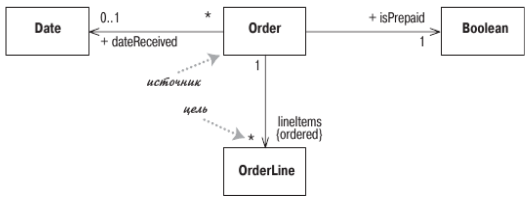
\includegraphics[width=0.7\textwidth]{associations.png}

					Ассоциации
				\end{center}
			\end{column}
		\end{columns}
		\bigskip
		Синтаксис:
		\begin{itemize}
			\item видимость имя: тип кратность = значение по умолчанию \{строка свойств\}
			\item Видимость: + (public), - (private), \# (protected), \char`~ (package)
			\item Кратность: 1 (ровно 1 объект), 0..1 (ни одного или один),\newline * (сколько угодно), 1..*, 2..*
		\end{itemize}
	\end{frame}

	\begin{frame}
		\frametitle{Агрегация и композиция}
		Агрегация – объект ``знает'' о другом (не управляет его временем жизни, имеет на него ссылку или указатель)
		\begin{center}
			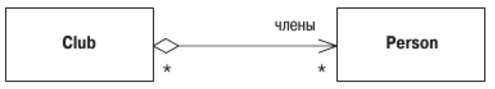
\includegraphics[width=0.5\textwidth]{aggregations.png}
		\end{center}
		Композиция --- объект владеет другим объектом (управляет его временем жизни, хранит его по значению или по указателю, делая delete)
		\begin{center}
			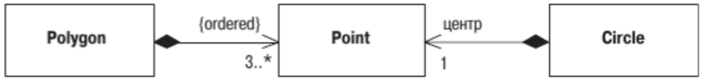
\includegraphics[width=0.7\textwidth]{compositions.png}
		\end{center}
		Уточнение обычной ассоциации, используется только если очень надо
	\end{frame}

	\begin{frame}
		\frametitle{Прочее}
		\begin{columns}
			\begin{column}{0.5\textwidth}
				\begin{center}
					Интерфейсы

					\bigskip
					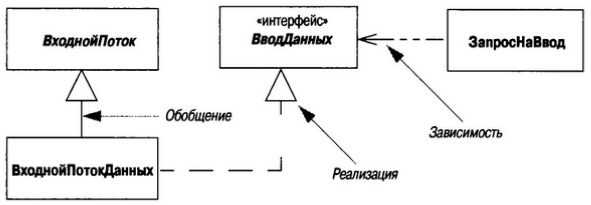
\includegraphics[width=0.9\textwidth]{interfaces1.png}

					\bigskip
					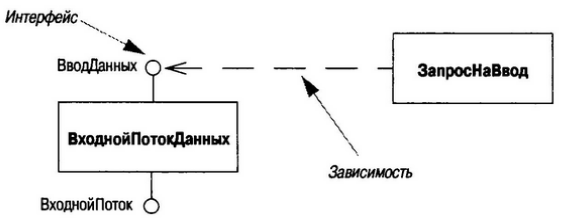
\includegraphics[width=0.9\textwidth]{interfaces2.png}
				\end{center}
			\end{column}
			\begin{column}{0.5\textwidth}
				\begin{center}
					Зависимости

					\bigskip
					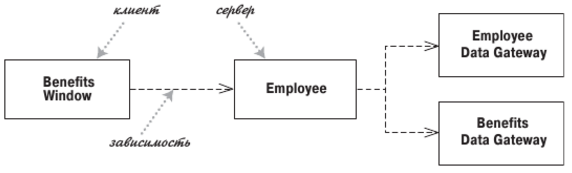
\includegraphics[width=0.9\textwidth]{dependencies.png}
					\bigskip

					Шаблоны

					\bigskip
					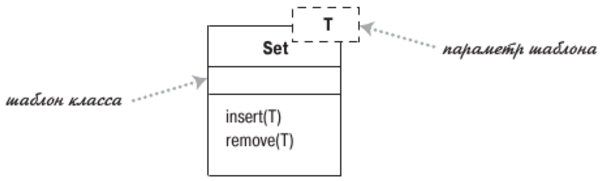
\includegraphics[width=0.9\textwidth]{templates.png}
				\end{center}
			\end{column}
		\end{columns}
	\end{frame}

	\begin{frame}
		\frametitle{Диаграммы объектов}
				\begin{columns}
			\begin{column}{0.5\textwidth}
				\begin{itemize}
					\item snapshot структуры классов во время выполнения
					\item Используются обычно чтобы пояснить диаграмму классов
					\item Полезны на этапе анализа предметной области, ещё до диаграмм классов
				\end{itemize}
			\end{column}
			\begin{column}{0.5\textwidth}
				\begin{center}
					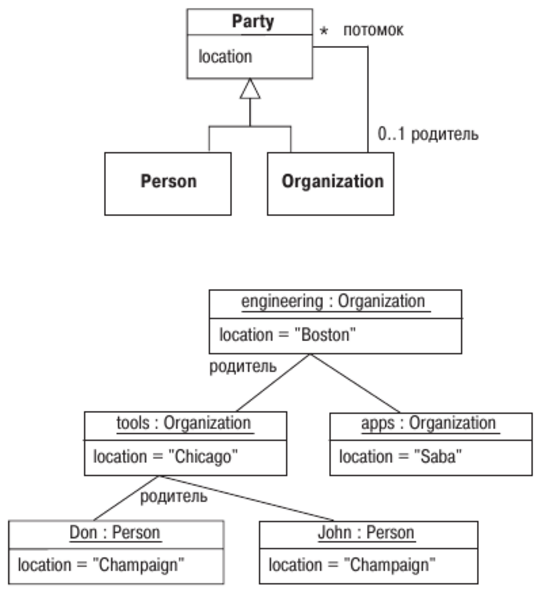
\includegraphics[width=\textwidth]{objectsDiagram.png}
				\end{center}
			\end{column}
		\end{columns}
	\end{frame}

	\section{Задания}

	\begin{frame}
		\frametitle{Домашнее задание 1: Магазин книг}
		Выполнить анализ предметной области и построить модель в виде диаграммы классов для интернет-магазина книг по следующему ТЗ:
		\begin{itemize}
			\item \url{https://goo.gl/94LyFc}
		\end{itemize}

		Обратите внимание, что это должна быть модель предметной области, детали реализации наподобие способа хранения информации в базе данных не важны.

		Будет оцениваться точность следования ТЗ, соответствие модели сущностям предметной области (в том числе, неявным) и, естественно, пунктуальность в следовании синтаксису UML.
		\bigskip
		Дедлайн: \textbf{29.03.2017г}.
	\end{frame}

	\begin{frame}
		\frametitle{Домашнее задание 2: cd, ls}
		\framesubtitle{Кое-что на ``покодить''}
		\begin{itemize}
			\item Реализовать команды \textbf{ls} и \textbf{cd} на базе кода одногруппника
			\begin{itemize}
				\item Обе команды могут принимать 0 или 1 аргумент
				\item Не забывайте про юнит-тесты
			\end{itemize}
			\item Написать ревью на архитектуру оного одногруппника, указав, что оказалось удобным, а что неудобным при реализации, что можно было бы улучшить
			\item Сделать fork на GitHub, выложить изменения туда и сделать пуллреквест в свой форк
			\begin{itemize}
				\item Если вы не стесняетесь и ``жертва'' не против, можно и в исходный репозиторий
			\end{itemize}
			\item Реализация, в которой надо сделать команды, определяется циклическим сдвигом на \textbf{3} вниз по списку на HwProj
			\item Дедлайн: \textbf{19.04.2017г}.
		\end{itemize}
	\end{frame}

	\begin{frame}
		\frametitle{Задание на остаток пары}
		\begin{itemize}
			\item Нарисовать диаграмму классов UML для своего решения CLI, как оно есть
			\item Обращать внимание на синтаксис UML и читаемость диаграммы
			\item Как будет готово, позвать меня и показать
			\item Не пытаться рисовать методы, кроме самых важных
			\item Не рисовать все поля, можно даже не рисовать все классы --- надо успеть до конца пары
		\end{itemize}
	\end{frame}

\end{document}
